\subsection{Konstruktion 1D}
Im Fokus der Konstruktionsansätze stand es, einen möglichst einfachen Aufbau zu entwickeln, der mit konventionellen Maschinen unter geringstem Einsatz fertigbar ist. Dies wurde durch die Verwendung von Standardmaterialien mit Standardmaßen erreicht, welche weit verbreitet sind. Weiter können alle Teile aus Blechen bzw. Stangenmaterial gefertigt werden, somit ist kein Einsatz von CNC Maschinen mit fünf oder mehr Achsen notwendig. In diesem Fall wurden 80 Prozent der Teile mittels einer Wasserstrahlschneidmaschine gefertigt. Der Einsatz von Passungen wurde auf das nötige Minimum reduziert. Aufgrund der Weiterverwendung dieses Projektes für eine Vorlesung, musste bei der Entwicklung darauf geachtet werden, das System möglichst wartungsfreundlich zu gestalten. Das gesamte Modell lässt sich in drei Baugruppen zerlegen, somit können alle Verschleißteile, wie z.B. Bremsbeläge und Lager schnell gewechselt werden. Aus Gewichtsgründen wurden alle Bauteile sehr schlank dimensioniert. 


\subsubsection{Bauteile}

Beim Bremsen drückt der Bremshebel auf die Schwungscheibe und presst diese gegen den unteren Bremsbelag. Dabei wird der Motorschaft radial belastet. Um diese Belastung zu verringern wird die Schwungmasse zusätzlich gelagert. Dies wird durch den Flansch mit Achse realisiert. In der Würfelseite ist ein Lager eingelassen, in dem die Achse des Flanschs geführt wird. 

	\begin{figure}[!h]
	\begin{center}
	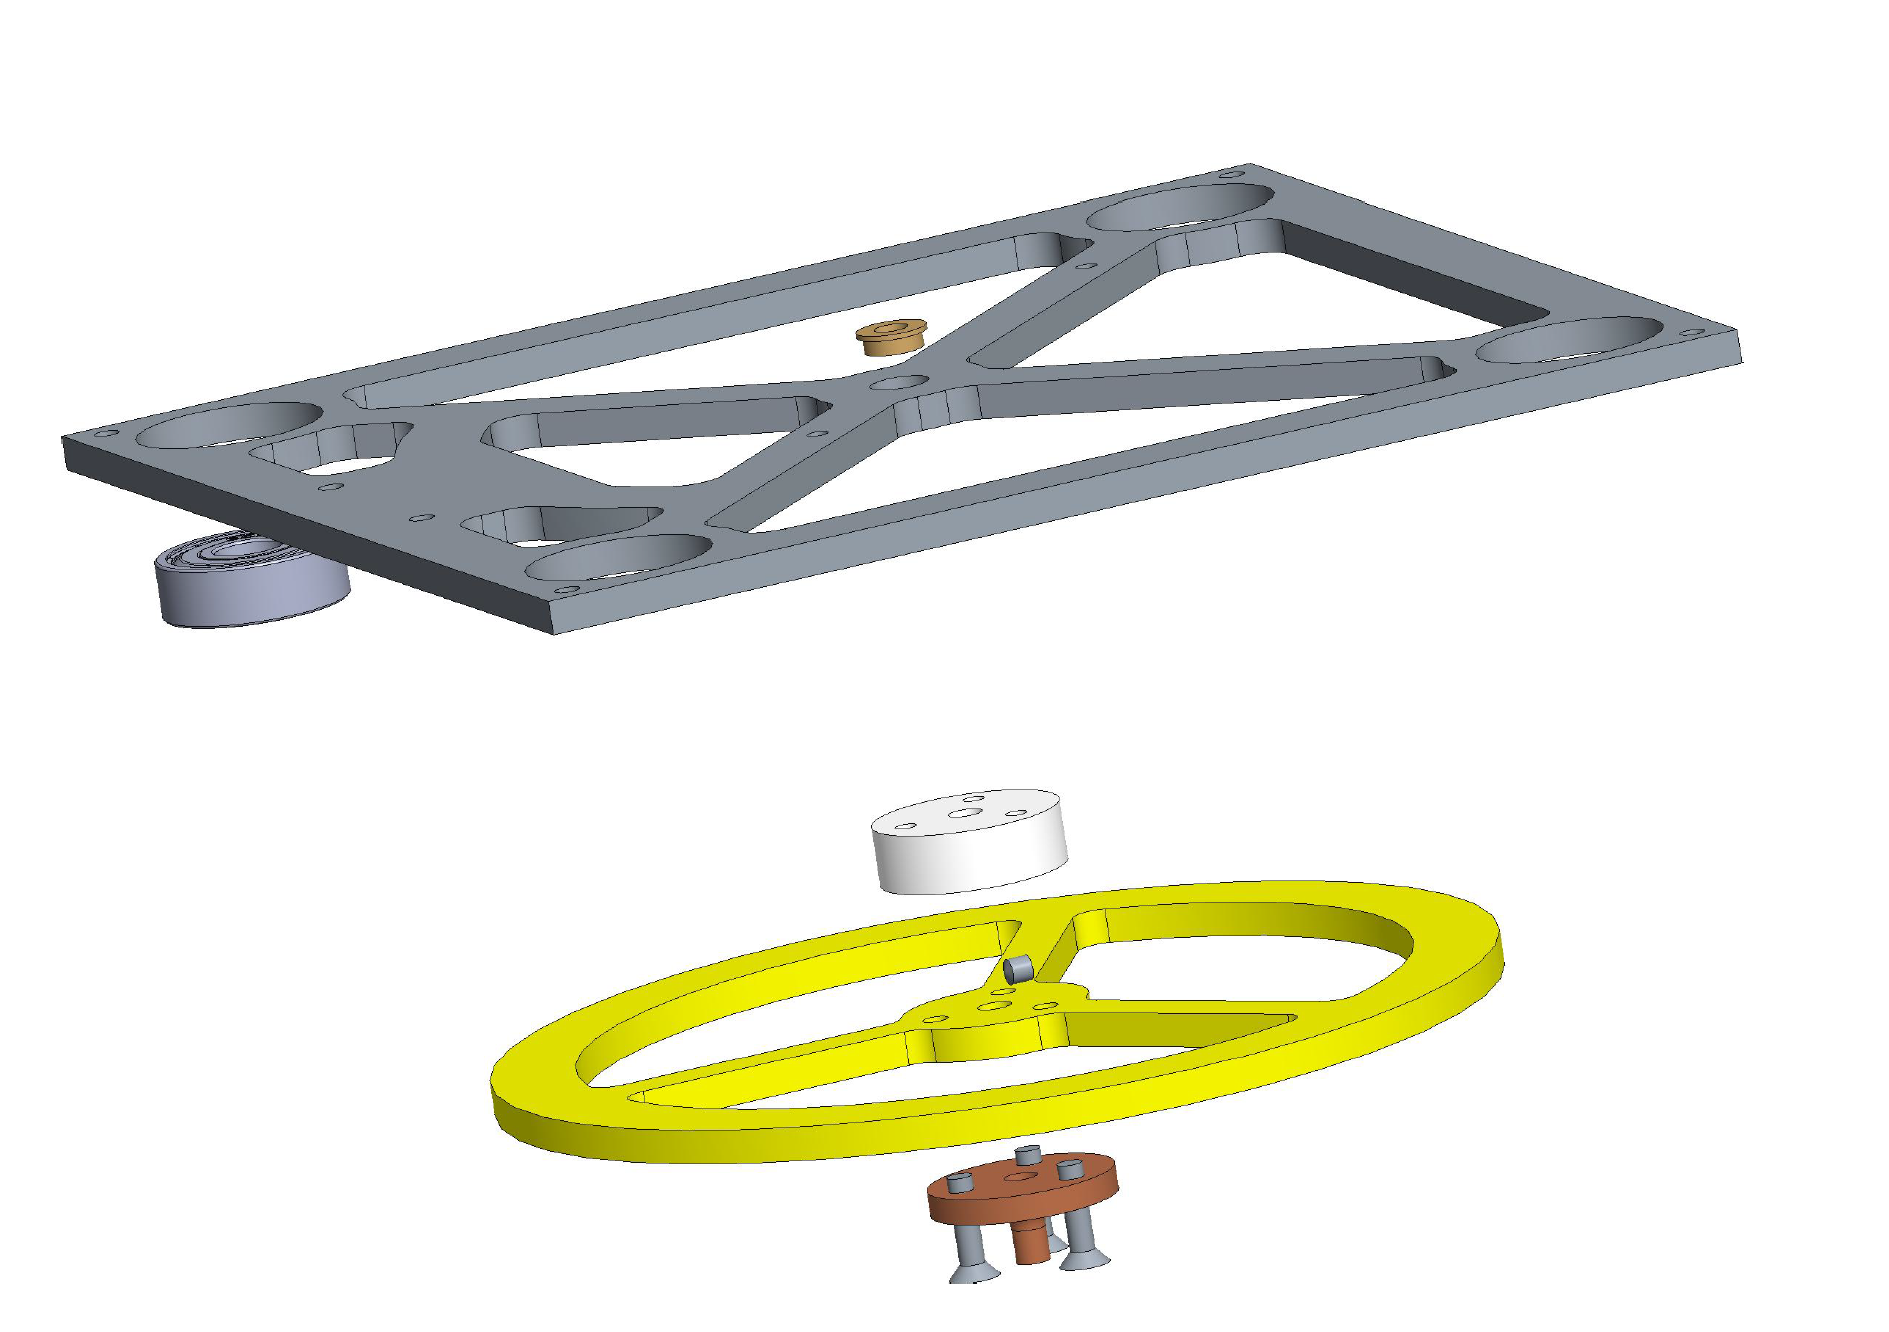
\includegraphics[width=0.75\textwidth]{img/Explosionszeichnung_Schwungscheibe.png}
	\end{center}
	\caption{Flansch Motorseite, Quelle: eigene Darstellung}
	\end{figure} 
 

	\begin{figure}[!h]
	\begin{center}
	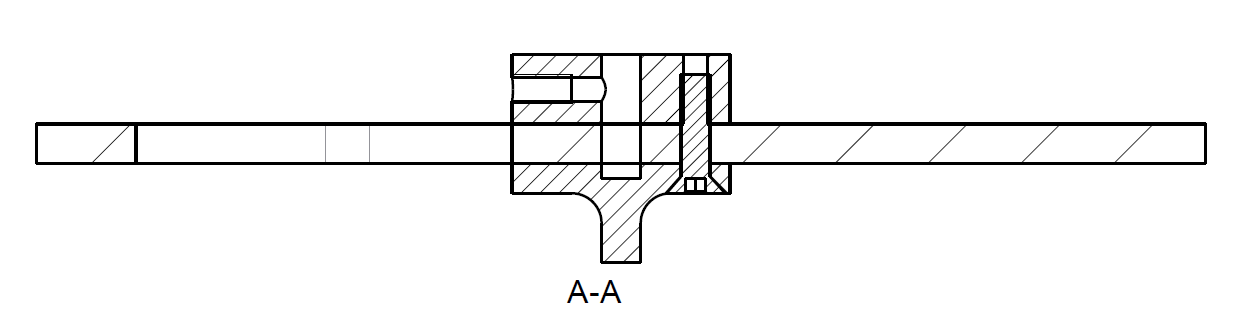
\includegraphics[width=0.75\textwidth]{img/Schwungmasse_mit_Flanschen_Schnitt}
	\end{center}
	\caption{Schnitt durch Schwungmasse mit beiden Flanschen, Quelle: eigene Darstellung}
	\end{figure} 

Der Motor selbst wird auf dem Motorhalter befestigt, welcher wiederum über die Halteplatte mit der Würfelseite verbunden ist. Am Motorhalter ist zusätzlich der Servo-Motor befestigt, der für die Aktuierung der Bremse notwendig ist. 
Im Hinblick auf die Konstruktion des gesamten Würfels, muss der Motorhalter zusätlich angepasst werden, so dass die Befestigung des Motors in zwei Richtungen erfolgen kann. Im Würfel würden drei gleiche Motorhalter dazu führen, dass die Bauteile sich gegenseitig im Weg stehen. 

	\begin{figure}[h!]
	\begin{center}
	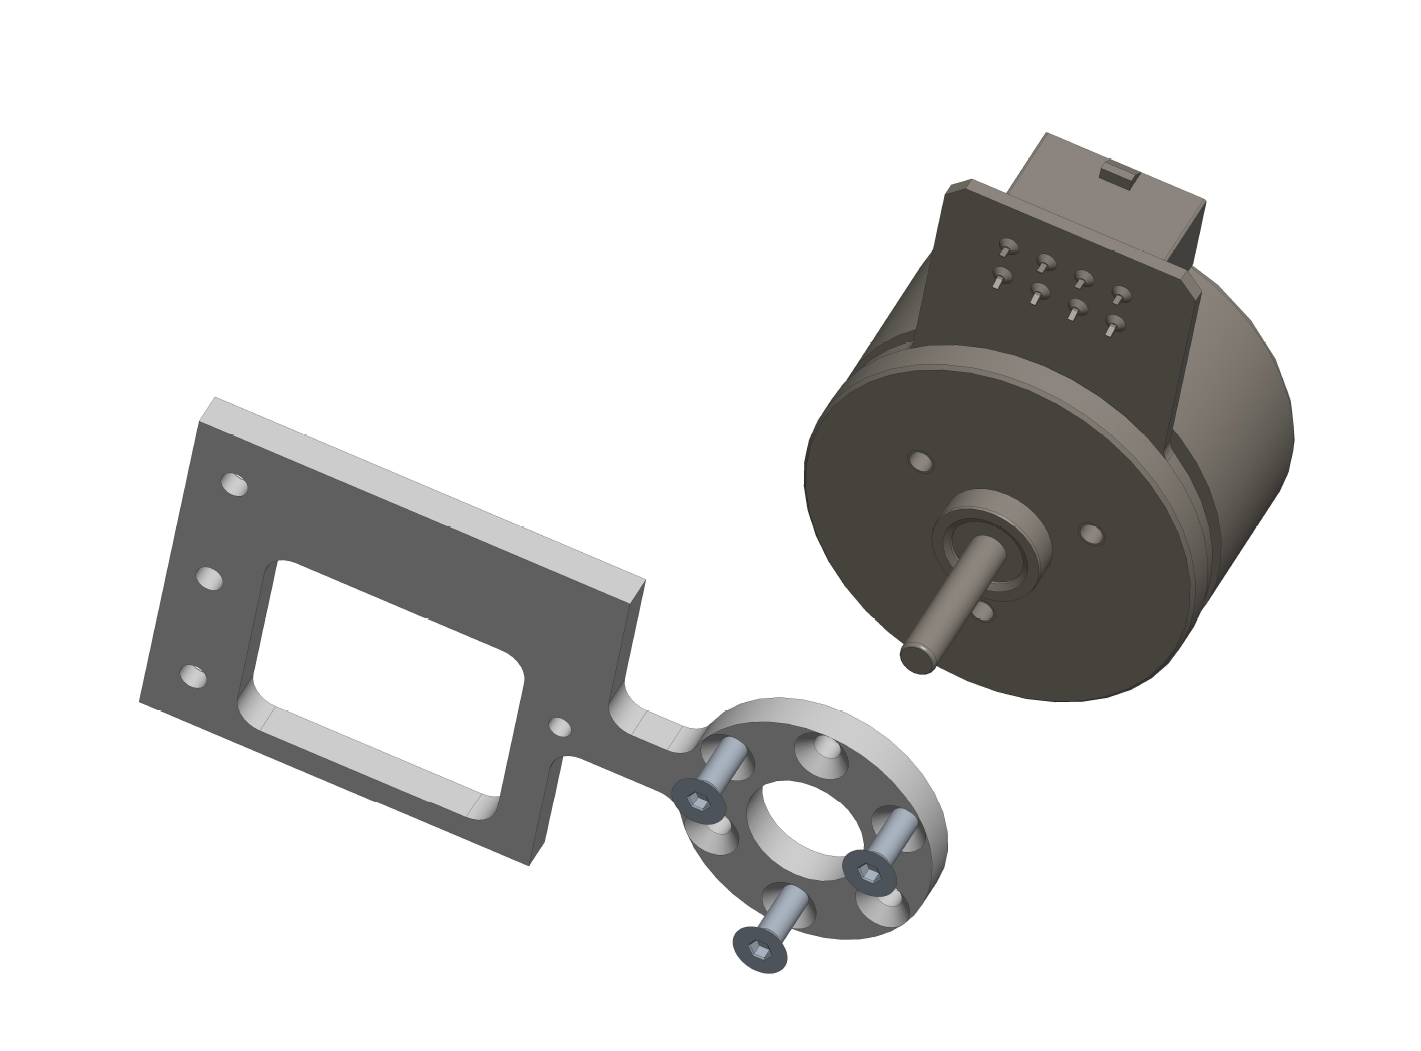
\includegraphics[width=0.75\textwidth]{img/Explosionszeichnung_Motor_Motorhalter.png}
	\end{center}
	\caption{Motorhalter, Quelle: eigene Darstellung}
	\end{figure} 

Die Bremse wird durch den Servo-Motor über das Servohorn nach dem Hebelprinzip bewegt. 


\begin{figure}[h!]
	\begin{center}
	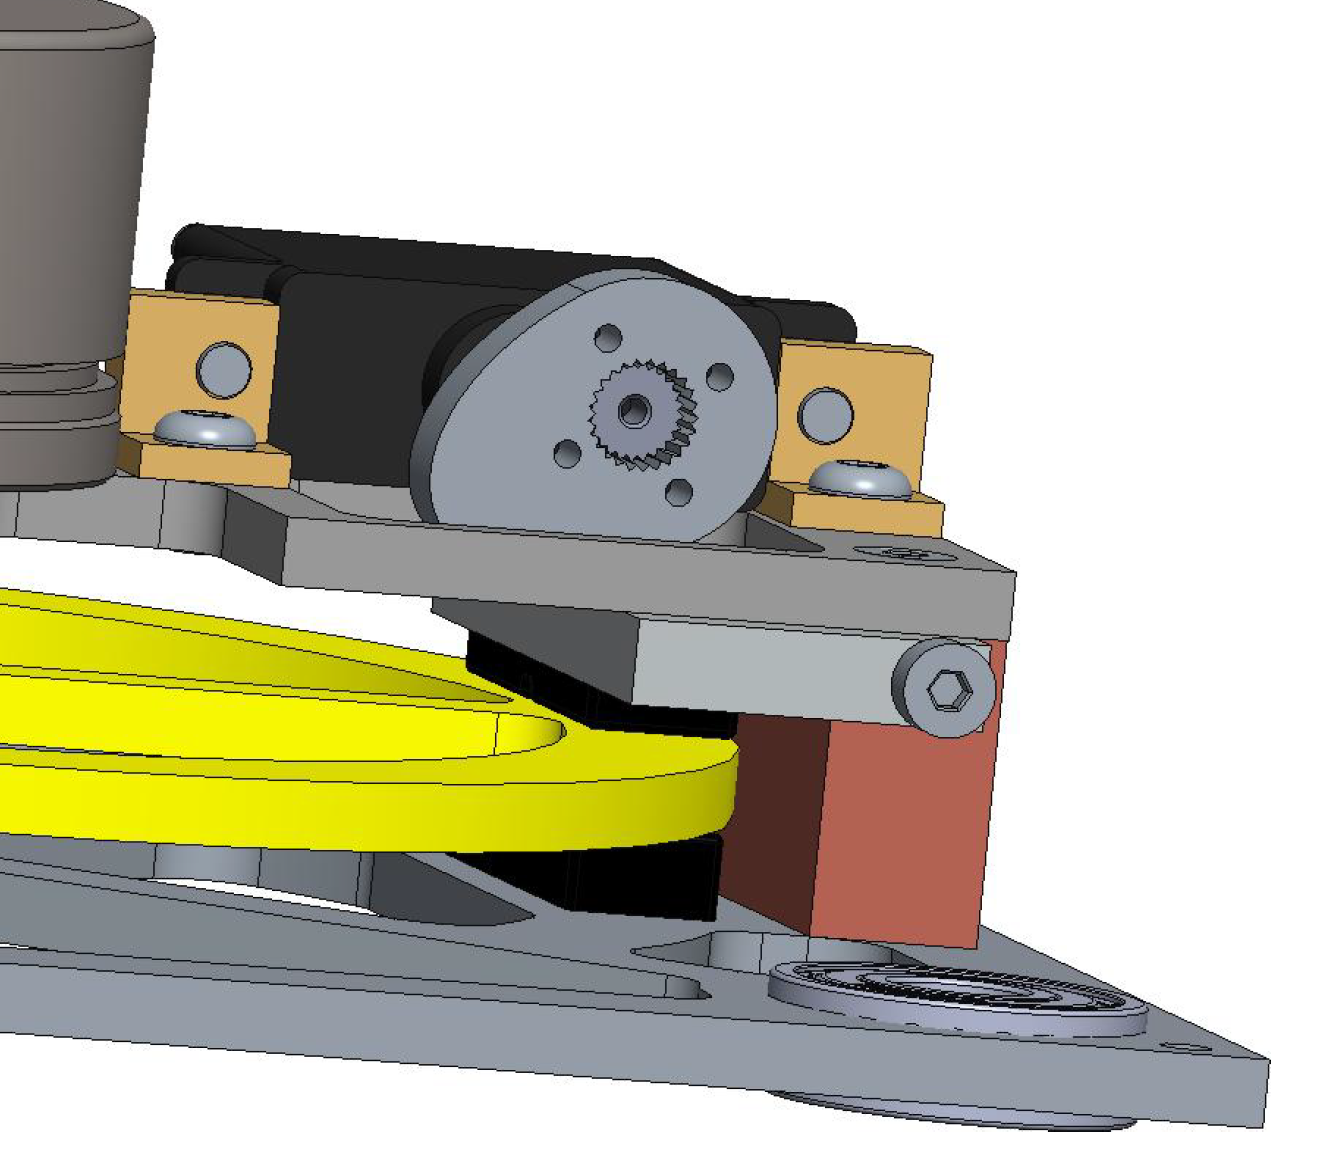
\includegraphics[width=0.75\textwidth]{img/Bremse_detail.png}
	\end{center}
	\caption{Bremsmechanismus, Quelle: eigene Darstellung}
	\end{figure} 

\newpage
Um die Komplexität des Systems vorerst zu vereinfachen, wurde diese Würfelseite zusammengebaut und in einer der Ecken gelagert um  Freiheitsgrade zu eliminieren. 
Die Bewegung kann somit nur noch in einer Ebene erfolgen. Von konstruktiver Seite wurden Aussparungen für ein 608ZZ-Lager vorgesehen. Über eine Achse, die fest gelagert wird, ergibt sich folgender Aufbau. 

\begin{figure}[h!]
	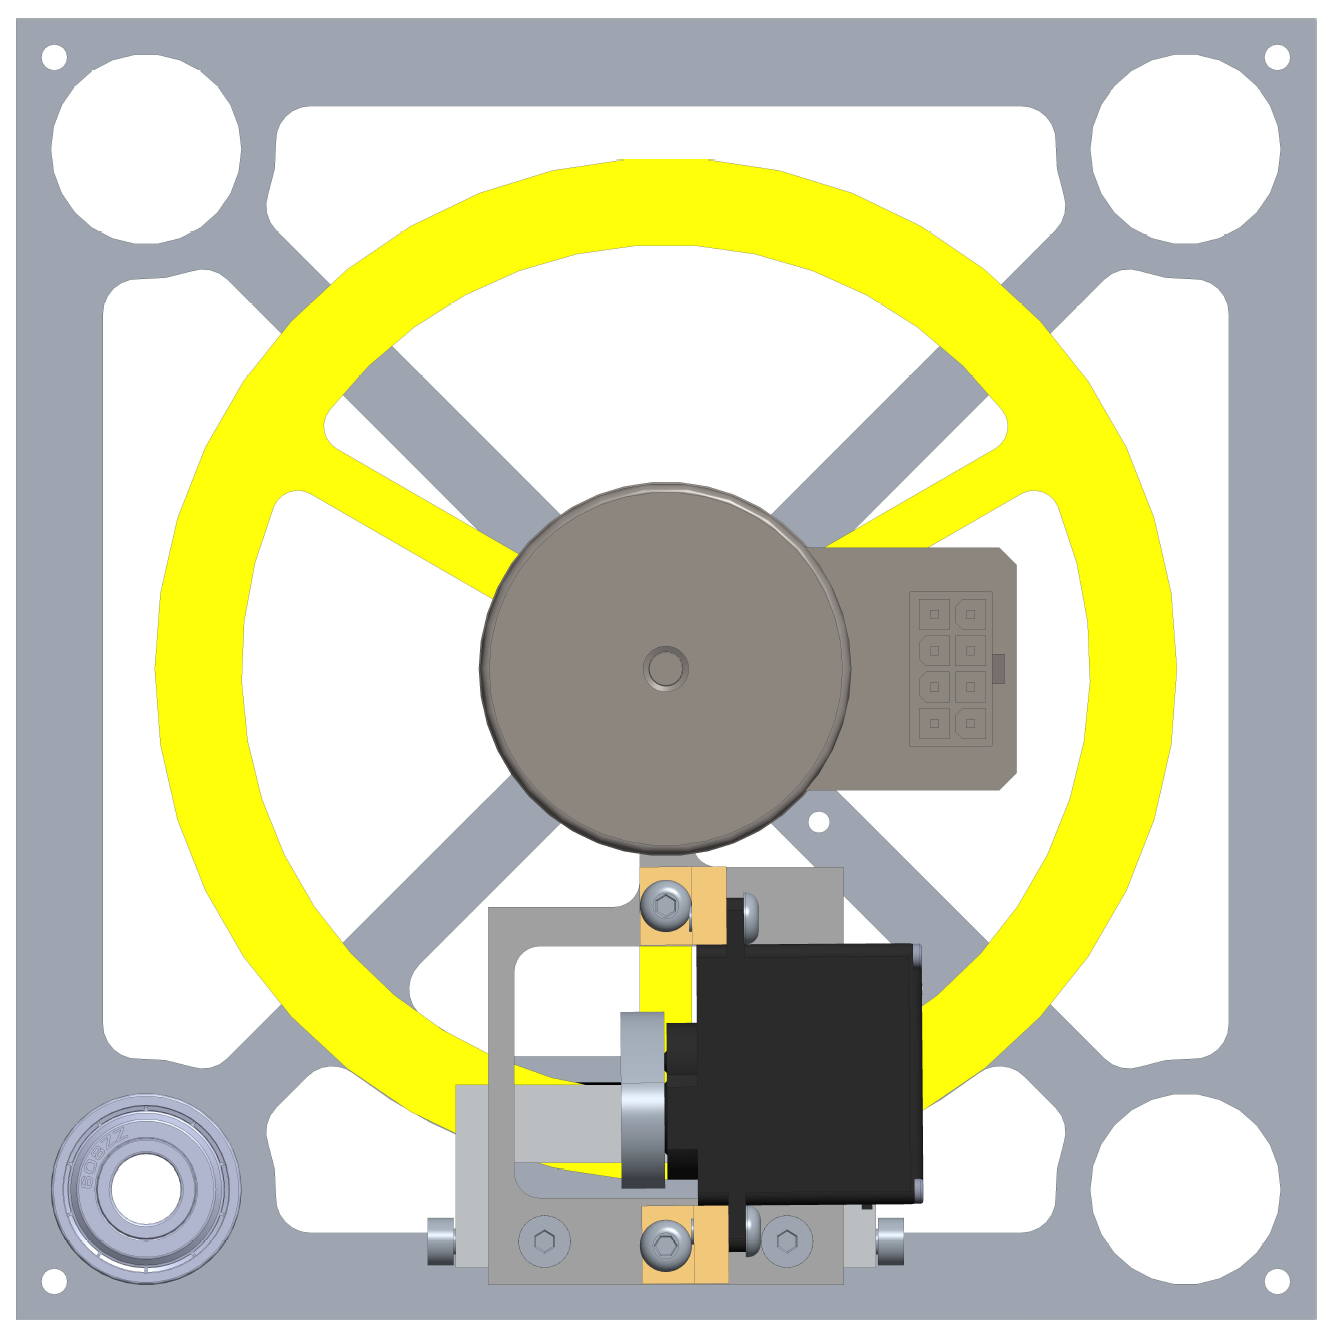
\includegraphics[width=0.49\textwidth]		  {img/1d_assembled_top}	   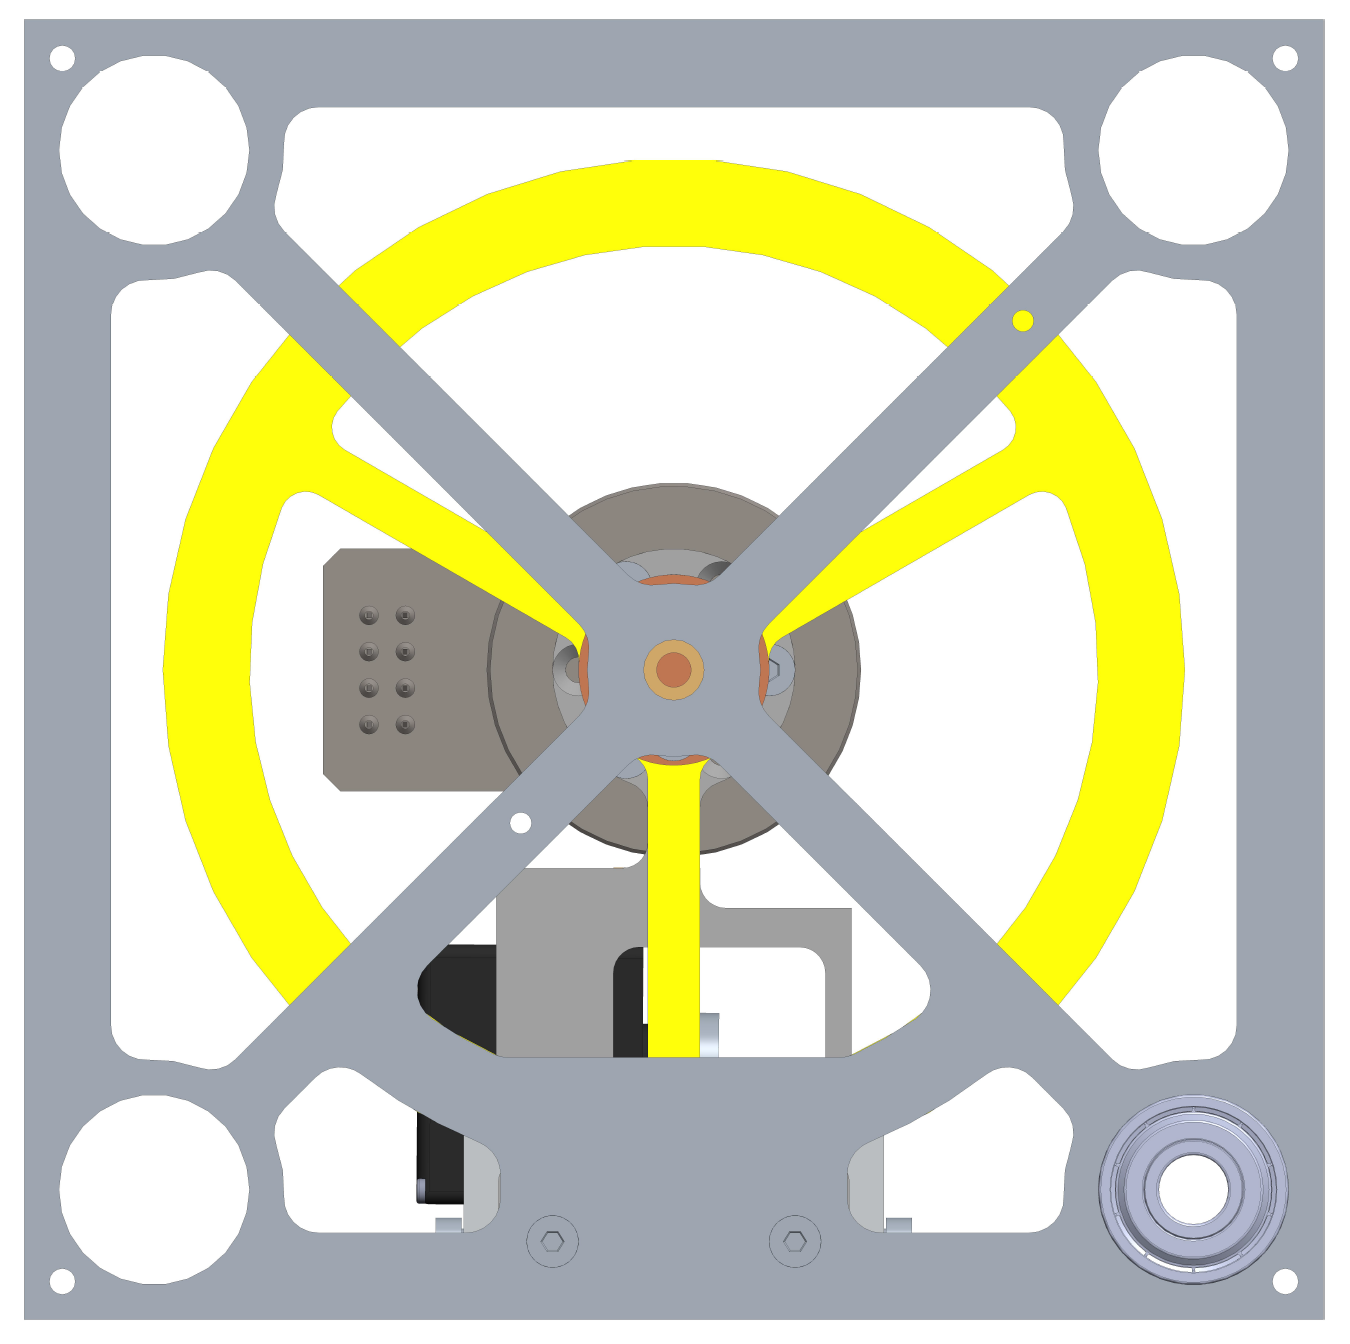
\includegraphics[width=0.49\textwidth]{img/1d_assembled_bottom}								\caption{Komplette Baugruppe, Quelle: eigene Darstellung} 
	\end{figure} 

\begin{figure}[h!]
	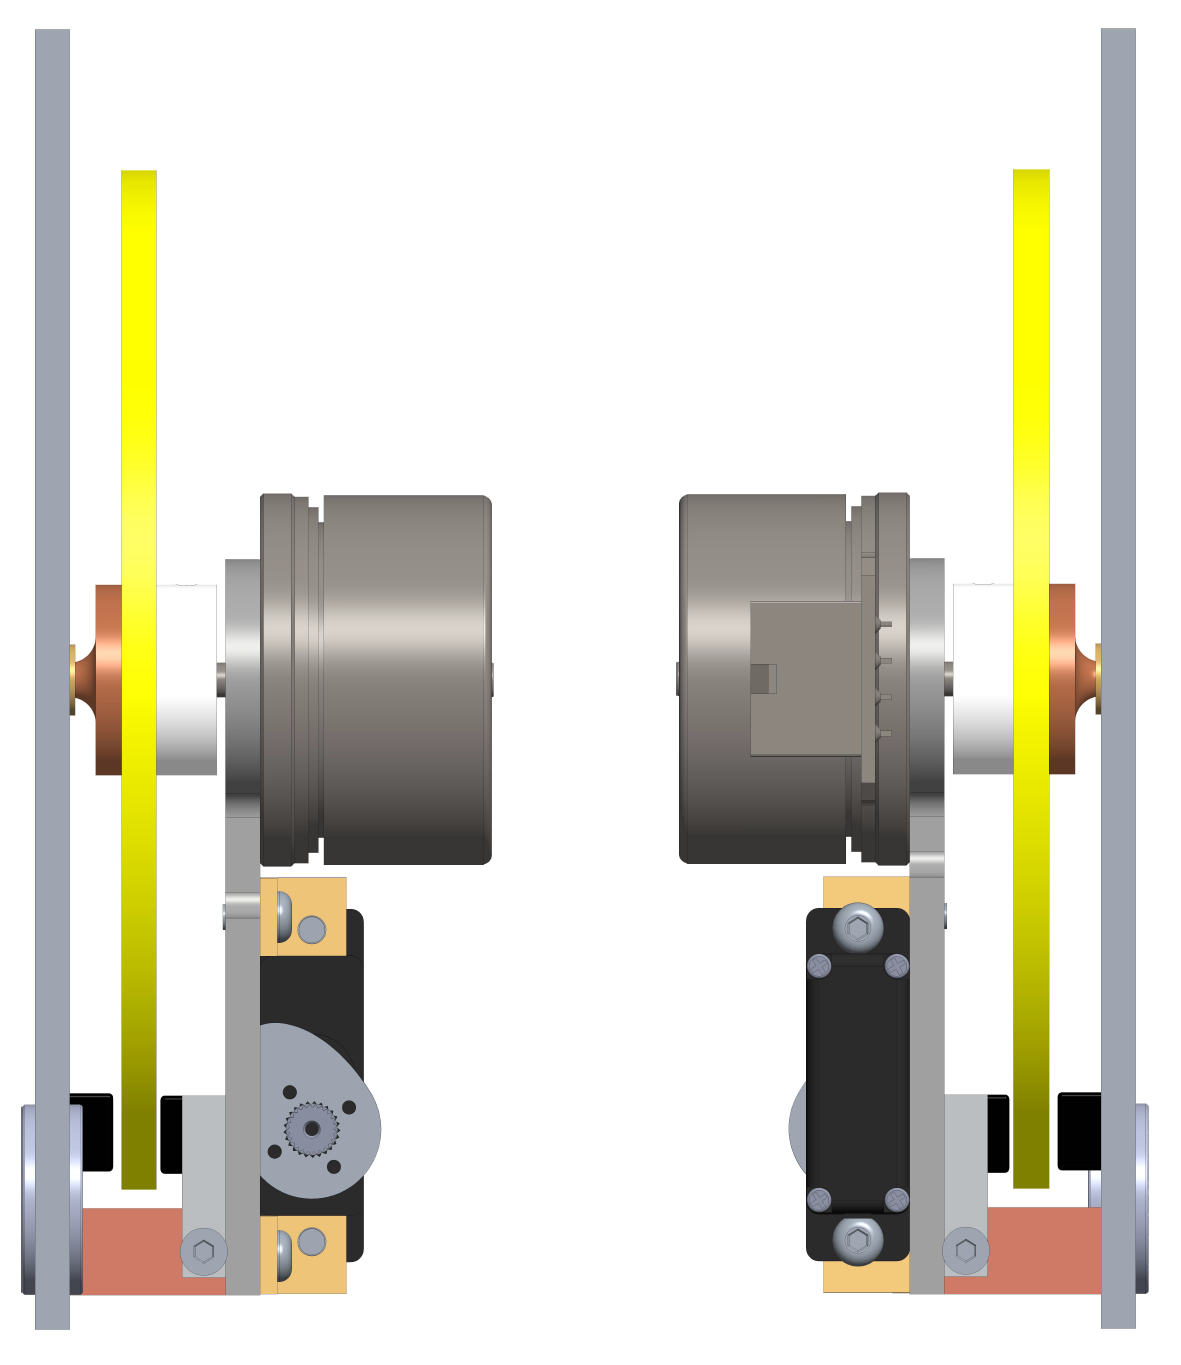
\includegraphics[width=0.49\textwidth]{img/1d_assembled_side}
	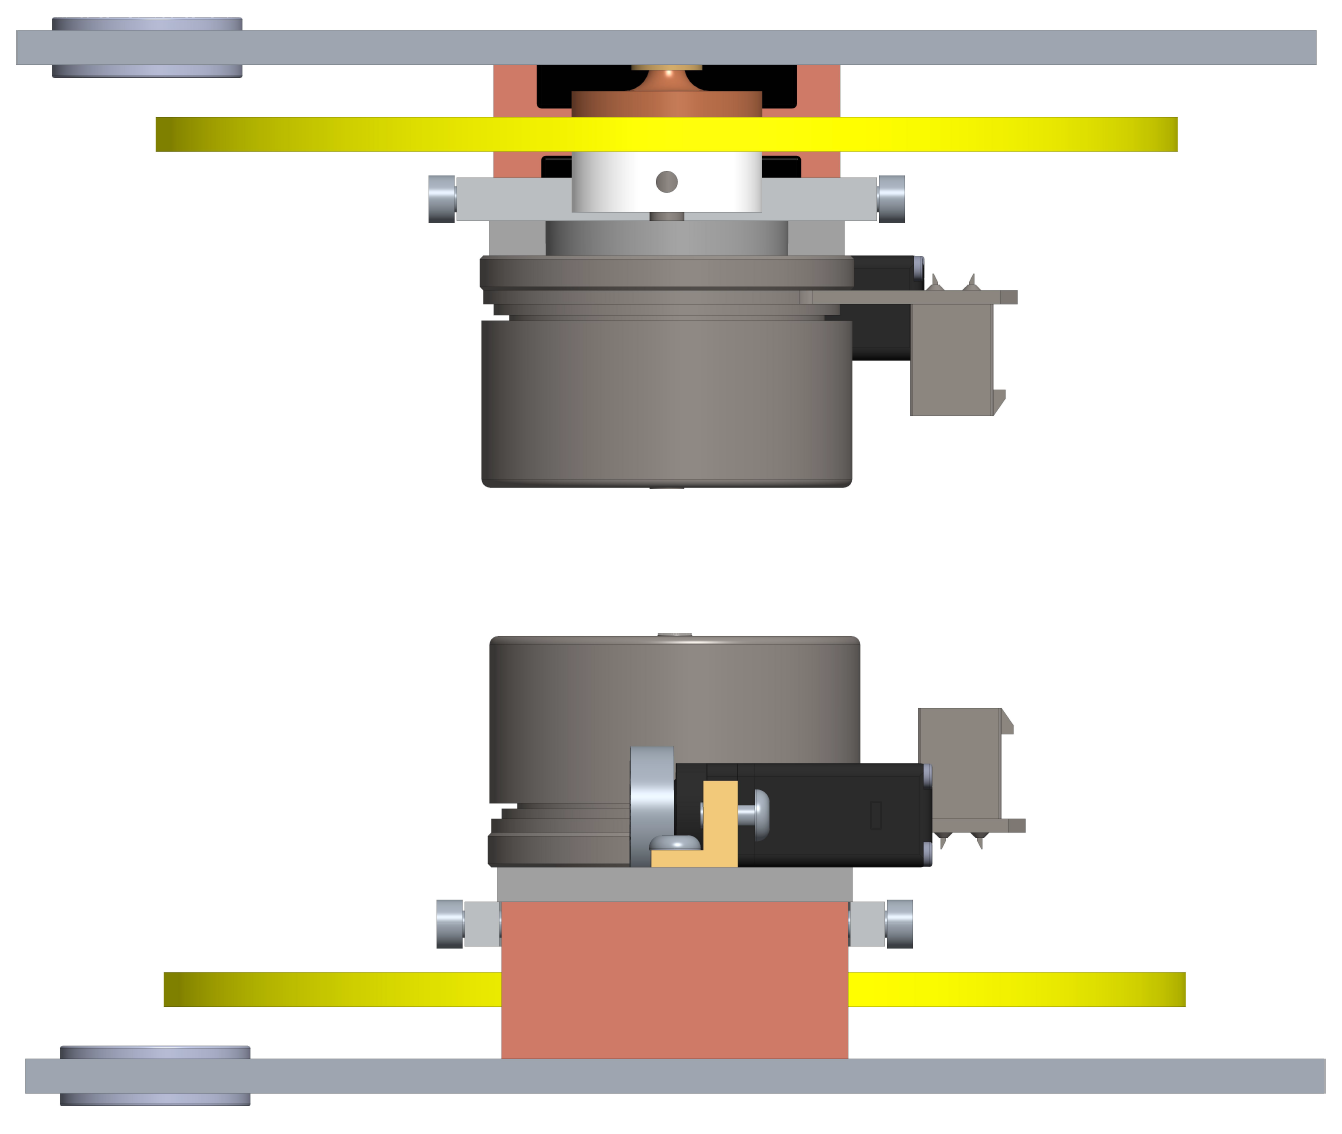
\includegraphics[width=0.49\textwidth]{img/1d_assembled_front_back}
	\caption{Komplette Baugruppe, Quelle: eigene Darstellung} 
	\end{figure} 

	\begin{figure}[h!]
	\begin{center}
	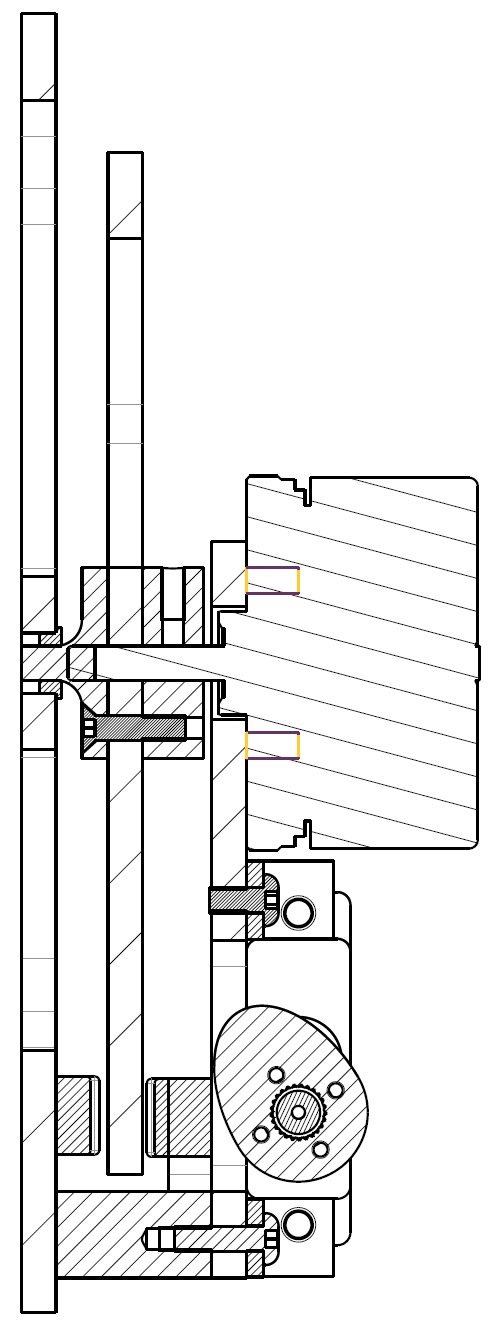
\includegraphics[width=0.4\textwidth,angle=90]{img/1d_assembled_schnitt}
	\end{center}
	\caption{Schnitt durch komplette Baugruppe, Quelle: eigene Darstellung}
	\end{figure} 
 

		
